% Chapter 1

\chapter{Introduction} % Main chapter title

\label{Chapter1} % For referencing the chapter elsewhere, use \ref{Chapter1} 

%----------------------------------------------------------------------------------------
% Define some commands to keep the formatting separated from the content 
\newcommand{\keyword}[1]{\textbf{#1}}
\newcommand{\tabhead}[1]{\textbf{#1}}
\newcommand{\code}[1]{\texttt{#1}}
\newcommand{\file}[1]{\texttt{\bfseries#1}}
\newcommand{\option}[1]{\texttt{\itshape#1}}

%----------------------------------------------------------------------------------------
% 
% \hajj{Chapter One introduces the topic of the thesis to the reader. The critical part of writing Chapter One is to establish the statement of the problem and research questions. Basically, you are justifying to the reader why it is nec- essary to study this topic and what research question(s) your study will answer. Usually, the topic is based around a particular problem area that you want to focus on. However, before you introduce the reader to the specific topic and problem, you have to first provide the reader with the broader context (the general problem) and consequences related to the topic. In other words, before you discuss the specific problem, you need to contextualize your topic within the larger problem. For example, you would first discuss the problems related to the topic.
% Chapter One of the thesis includes a section on the Statement of the Problem (information about the specific problem), Background and Need (the background literature related to the problem), the Purpose of the Study (the focus and goal of the study), Research Questions (what questions the study proposes to answer), and other significant sections. In this chapter, you need to support all of your claims and positions using citations
%  check this reference please:
%  https://www.wcupa.edu/business-publicManagement/geographyPlanning/documents/thesisGuideline.pdf}
% \begin{enumerate}
    %item state the general topic and give some background
    %\item provide a review of the literature related to the topic
        % \item define the terms and scope of the topic
        % \item outline the current situation
        % evaluate the current situation (advantages/ disadvantages) and identify the gap
    % \item identify the importance of the proposed research
    % \item state the research problem/ questions
    % \item state the research aims and/or research objectives
    % \item state the hypotheses. DONE
    % \item outline the order of information in the thesis. DONE
    % \item outline the methodology. DONE
% \end{enumerate}


% General Research topic 
\section{Research Topic}We are in an era where it is difficult for industries and organizations to run a business process without connectivity and data exchange. With the advent of Industry 4.0, Digital Twins(DT) and Internet of Things(IoT) are the two enabling technologies that provide unprecedented levels of connectivity and data exchange to monitor and optimize business operation. Both technologies have been around for a while, but the integration of of them is just getting started.

\section{Literature Review}
...

% Niche
\section{Niche and Scope}
Internet of Things (IoT) is a network of physical objects, such as smart devices, sensors, actuators, vehicles and buildings powered by software and network connectivity that allow them to collect and exchange data[\textcolor{red}{ref}]. Digital Twin can be describe as software defined digital representation of physical object. It receive large set of sensor data about environment and operating condition to simulate and monitor operation in real-time[\textcolor{red}{ref}]. Simulation of an operation, visualization of product in real-time, trouble shooting remote equipment, managing assets in industry are few of the use cases amon the others[\textcolor{red}{ref}]. Together, those two technologies are transforming the way we manage resources and operations. 

% The importance of this research
% The challenge in story telling scenario 
\section{Importance of the Research}
Digital Twin and IoT have an important role to play in various sectors including industries, critical infrastructures, health, smart cities, and so on. Therefore, during the interaction or communication, it is important to ensure the security of those two technologies. Authentication is a critical security principle that can come to rescue to address the aforementioned concern by only allowing an authorized end point to access system and data. In other words, in context of Digital Twin and IoT, authentication can enable us to make sure only known IoT device can send sensor data to Digital Twin hub and only known Digital Twin send command to device situated remotely. Without authentication, a malicious user can gain access to a system, leading to serious security problems. 

\
% Problem statement 
\section{Problem Statement}
As noted previously, manufacturing facilities, including critical infrastructure, are using an IoT device to collect and send sensor measurement and operating conditions to the Digital Twin station to monitor and optimize the overall operation of the business process. However, due to the storage and processing constraints that IoT devices have [ \cite{williams_survey_2022}, \cite{noauthor_lightweight_nodate}], it is challenging to adopt traditional security cryptographic mechanisms to ensure the confidentiality and integrity of the data flow between IoT and DT. If proper security measures (authentication, authorization, encryption, and so on) are not used, an attacker may be able to perform a man-in-the-middle attack with the intent of intercepting sensitive sensor data or disrupting a system by injecting his crafted faulty data[\textcolor{red}{ref}]. In recent literatures and blog of standard institutes, it is mentioned to utilize security schemes that can fit into constraint devices to address the security requirement.  

% Proposed Solution and Hypothesis 
\section{Proposed Solution}
In this study, we propose a lightweight mutual authentication scheme , based on NIST standardized authentication encryption, to ensure the security requirement of IoT applications and Digital Twin. Our authentication scheme will enhance the confidentiality and integration of the communication channel between the Digital Twin and its counter physical component. In addition, we envision that our mutual lightweight authentication scheme can also provide secure access to remote IoT device(sensors) and  Digital Twin station. 

\section{Research Objective and Aims}
This research has two main objectives. First, through systematic literature review, analyze the core concept of a Digital Twin and synthesis the information presented in the literature on how DT is used to enhance the security of IIoT/IoT application in industry 4.0 use cases. Second, with the objective of implementing NIST standard light-weight authentication scheme, we aim to improve the security of a digital communication that is established between power, storage, and processing constraint devices and DT statation hosted on cloud or local premises. In the context of industry 4.0 uses cases,  IIoT devices are field devices such as sensors and actuators situated in a remote industry zone where it is not convenient to reach and access them. Hence, it is important to implement an efficient and performant cryptographic solution to increase the life-longevity of these power constraints devices to avoid periodic repairs or replacement.  

\section{Hypothesis}
% More security
% efficiency increase speed of data flow 
% Getting a real time of data is one requirement of DT application 
Getting real-time and authentic data from sensors is one requirement of DT application[\textcolor{red}{ref}].In this sense, implementing a lightweight authentication scheme will enhance security and increase the speed of data flow between DT and IIoT sensors. In addition, our scheme can provide remote secure access to IoT and DT.  


% Methodology 
\section{Methodology}
This study has two major part;literature review and implementation of proposed solution. For the literature review, we conducted a systematic way of reviewing previous leiteratures with the aim of synthesizing the core concept of Digital Twin and analyzing the existing solution for securing IoT application using Digital Twin. To implement our proposed solution, which is a lightweight authentication scheme, we leverage platform called Ditto and microcontroller manufactured by Pycom called ESP32. Ditto is an open source framework developed and maintained by Eclipse Foundation to facilitate the interaction between Digital Twin and IoT devices\cite{noauthor_eclipse_nodate}.ESP32 microcontroller is a chipset that can be programmed with micropython which is an implementation of Python3 for microcontroller. 
The performance and efficiency of our proposed solution is validated, at the end of the study, by measuring the power consumption, execution time, and storage complexity. 

\begin{figure}[h!]
    \centering
    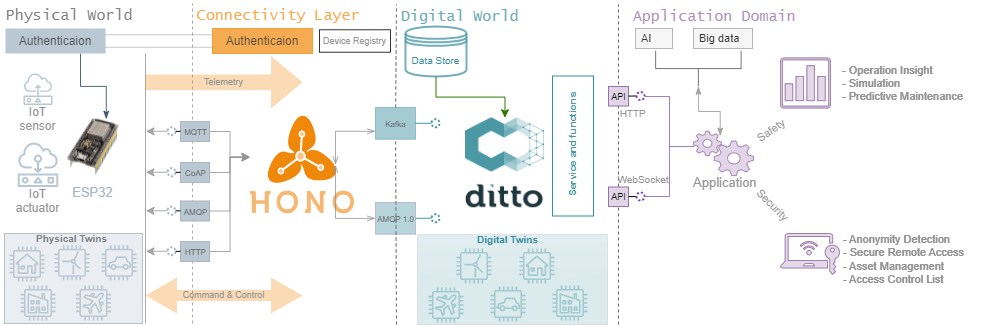
\includegraphics[width=1\textwidth]{images/ps-scheme2.png}
    \caption{Proposed solution schemes and experiment context}
    \label{fig:ps-scheme}
\end{figure}

% outline the order of information in the thesis 
\section{Report outline}
The remainder of this study report is organized as follow. In the following section, we present the methodology we imploy for the systematic literature review process. Then we provide details of the results of the literature review. Following that, we discuss the summary of the result and limitations of the study. Finally, we draw our conclusion on the basis of the evidence we gathered.   

% The emergence of Digital Twins(DT) and the Internet of Things(IoT) has opened up a new opportunity for businesses to take advantage of technology to gain insights and optimize performance. To maintain the security and privacy of data, these technologies come, however, with their own unique set of security challenges that must be addressed. In this paper, we will explore the current state of security, particularly the authentication scheme used to ensure the confidentiality and integrity of data flow between the virtual model;the digital twin, and the physical devices, which could be sensors or actuators. We will also provide lightweight DT based authentication scheme along with how to implement for IoT application. Finally, we will conclude our work with a recommendation on how to protect a DT and IoT network with efficient and performant cryptographic authentication schemes.

